\section{Numerical demonstration and comparison with a spiral planner}
\label{sec:demonstration}
\subsection{Matched vehicle, gravity and boundary conditions}
The following examples use the ship in the companion manuscript \cite{companion}: useful jet power $P=1\,\mathrm{GW}$, initial mass $m_0=3\times10^6\,\mathrm{kg}$ and dry mass $m_*=10^6\,\mathrm{kg}$. Thus
\begin{equation}
 B=2P(1/m_*-1/m_0)=1333.333333\,\mathrm{m^2\,s^{-3}}.
\end{equation}
The engine is ideal and uncapped; no finite exhaust-speed band is imposed. Both methods start in a prograde circular orbit $100\,\mathrm{km}$ above the Moon and finish in a prograde circular orbit $200\,\mathrm{km}$ above Mars, with free orbital phase. They share the same prescribed coplanar ephemerides, launch instant and quadratic budget. The final propagated mass is approximately $1{,}000{,}000.067\,\mathrm{kg}$ in each case.

For the Solar-System example, Earth and Mars have circular heliocentric orbital radii $1$ and $1.523679\,\mathrm{AU}$; Mars initially leads Earth by $30^\circ$. The Moon starts $90^\circ$ from the common inertial $x$ axis at a geocentric distance of $384{,}400\,\mathrm{km}$. Angular velocities follow the stated circular-orbit model, and SOIs use $r_{\rm SOI}=a(\mu/\mu_{\rm parent})^{2/5}$. This is a specified launch geometry, not a dated ephemeris prediction. Local motion uses central gravity of the active body, with physical position and velocity matched at each moving SOI. These are the translating-centre patched equations discussed earlier, not a smooth simultaneous many-body integration.

\subsection{What the game comparison includes}
The supplied \texttt{TheLongBurn.zip} implements the local law
\begin{equation}
 \mathbf a_T=\sigma A\frac{\mathbf v_{\rm rel}}{\norm{\mathbf v_{\rm rel}}},
 \qquad \sigma=+1\ \hbox{(escape)},\quad -1\ \hbox{(capture)},
 \label{eq:game-law}
\end{equation}
in \texttt{tlb\_transfer/src/spiral.rs}; $A$ is constant and the effort is $A^2T$. Here ``tangential'' means along velocity, not necessarily the transverse polar direction on an eccentric trajectory. Capture is generated by backward integration from the final circular orbit. The planner's default arrival/departure acceleration ratio is one \cite{longburn}.

For a moon-to-another-planet transfer the planner also introduces a circular staging orbit about the departure planet. We reproduce the five-phase family: Moon escape, a flexible Earth-centred connector ending on the staging circle, constant-$A$ Earth escape, a flexible heliocentric leg, and constant-$A$ Mars capture. The staging radius is $a_M+1.5r_{{\rm SOI},M}$ when this is at most $0.8r_{{\rm SOI},E}$; the source's inner alternative applies otherwise. Here the outer choice is valid in both examples. We retain the Earth connector's two-planet-radius exclusion and its duration range of $0.01$--$1$ lunar periods.

The dashed curves are a \emph{reoptimized source-law family}: the shared $A$, spiral orientations, connector controls and transition times are optimized jointly. Reusable one-parameter spiral maps reduce this solve to two flexible legs; the selected spirals are then reintegrated directly. This is a Python reimplementation of the source's steering and staging restrictions, not a run of the Rust planner's coarse searches, phase-alignment heuristics or runtime. It is consequently a controlled comparison of trajectory families, not a benchmark of the game executable. The baseline can have thrust jumps at joins. The flexible four-phase candidate has no compulsory staging circle and permits radial and transverse thrust modulation; thrust-vector continuity is enforced at its physical SOI joins before small feasibility corrections.

\subsection{Acceleration zooms and reference frames}
Figure~\ref{fig:moonmars-comparison} adds local trajectory views, departure and arrival acceleration zooms, and a decomposition of the final capture thrust. All magnitude panels plot
\begin{equation}
 q(t)=\norm{\mathbf a_T(t)},
\end{equation}
not $\norm{\mathbf g+\mathbf a_T}$. The same physical thrust vector has the same norm in heliocentric or body-centred axes, including after a rotation of the plotting axes. A coordinate acceleration in an accelerating frame would require the inertial terms, but that is not the quantity plotted here. The radial/transverse components use the instantaneous local basis $(\mathbf e_r,\mathbf e_\theta)$ and therefore do depend on that rotating basis. The magnitude oscillations cannot be explained away by that rotation.

On a smooth unconstrained ideal PMP arc, the primer equations give
\begin{equation}
 \ddot{\mathbf a}_T=G^T\mathbf a_T,\qquad
 G=\frac{\mu}{r^3}(3\mathbf e_r\mathbf e_r^T-I).
\end{equation}
Writing the inertial direction rate of nonzero thrust as $\omega_a$ and its angle to $\mathbf e_r$ as $\gamma$ yields
\begin{equation}
 \ddot q=q\left[\omega_a^2+\frac{\mu}{r^3}(3\cos^2\gamma-1)\right].
\end{equation}
This displays the coupling of thrust modulation to the gravity gradient and changing geometry. It does not predict a universal oscillation period or prove that the finite-dimensional, feasibility-corrected trajectories exactly satisfy the continuous PMP. The plotted modulations are smooth and resolved under mesh refinement. Capture zooms align each method to its own arrival time, rather than comparing unequal physical flight phases at the same elapsed time.

\begin{figure*}[!t]
\centering
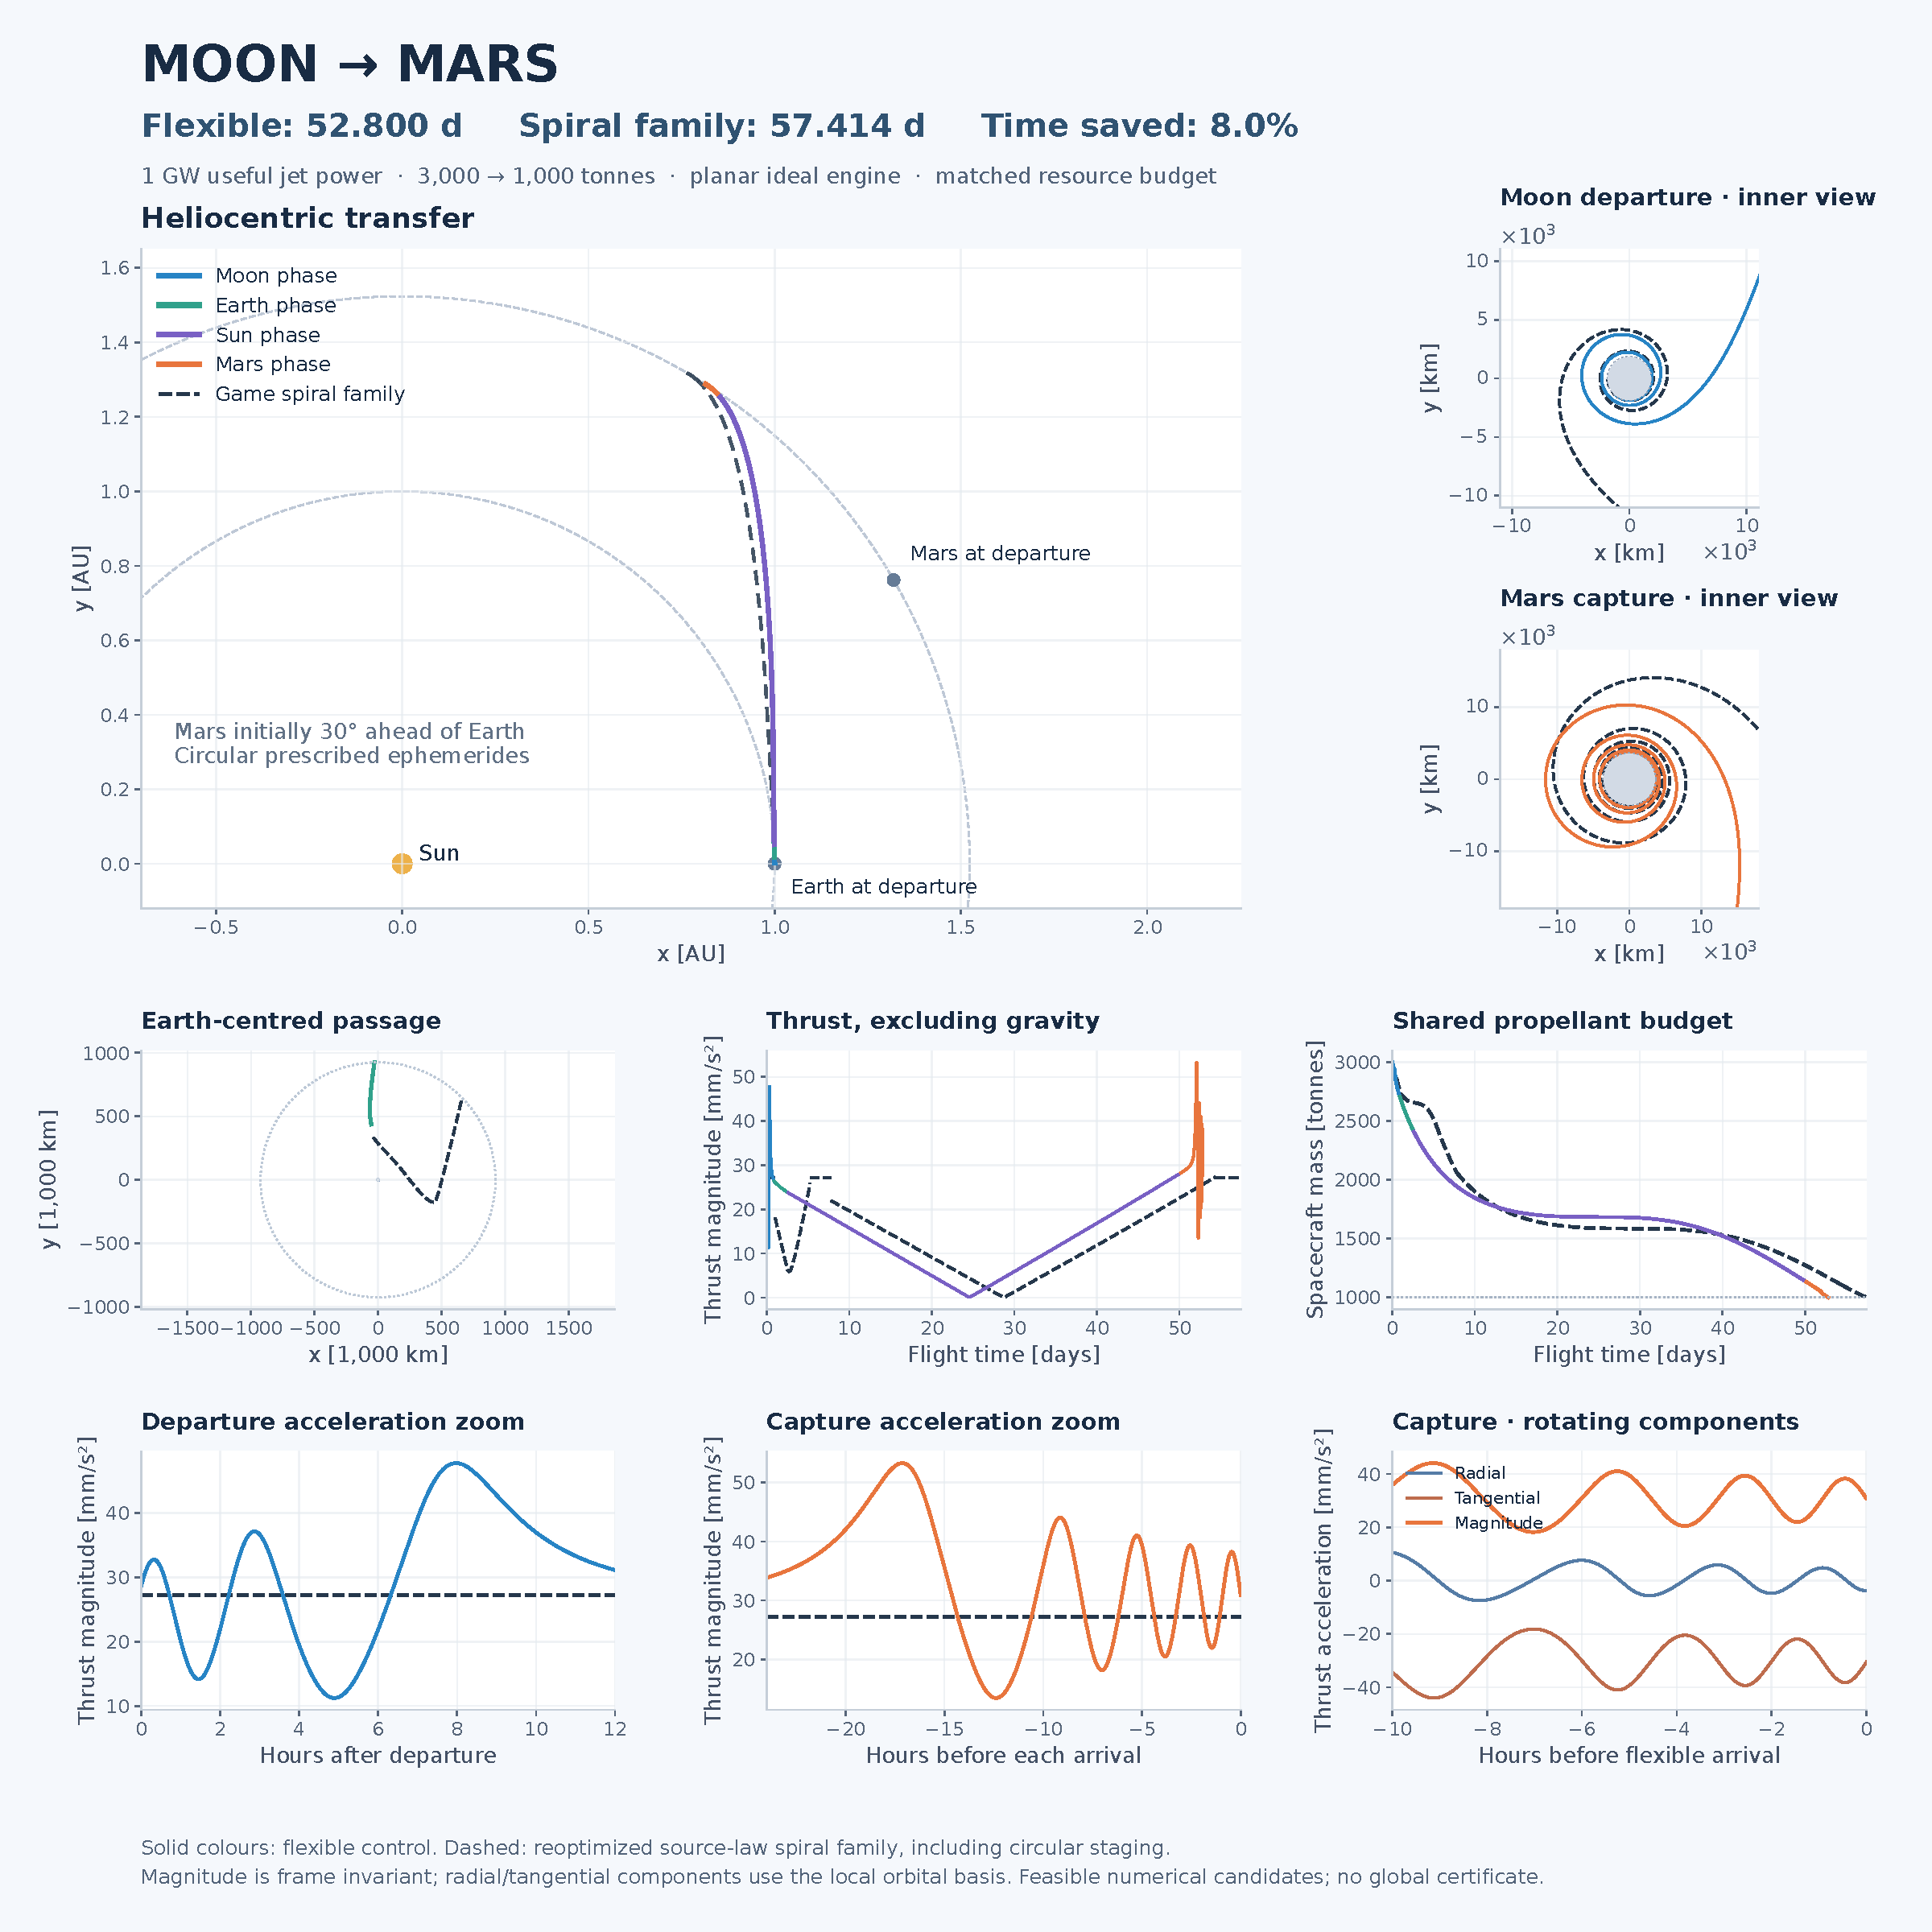
\includegraphics[width=\textwidth]{figures/moon_mars_comparison.pdf}
\caption{Matched Moon-to-Mars comparison. Solid phase colours show the flexible candidate; dashed curves show the reoptimized constant-acceleration spiral-and-staging family. The bottom row resolves the first $12$ hours of lunar departure, the last $24$ hours of Mars capture, and the last $10$ hours of capture components. The two methods choose their own free parking-orbit phases. The norm oscillations are physical thrust modulation, whereas the signed components are expressed in the rotating local orbital basis.}
\label{fig:moonmars-comparison}
\end{figure*}

\subsection{A constructed configuration with a larger gap}
To make local-leg restrictions more consequential, keep the Sun and ship unchanged and multiply each Earth, Moon and Mars analogue's mass by $s=0.003$ and radius by $s^{1/3}$ (unchanged mean density). Put the planetary analogues on circular $1$ and $1.006\,\mathrm{AU}$ orbits, initially aligned. Their heliocentric speeds are $29.7847$ and $29.6957\,\mathrm{km\,s^{-1}}$. Scale the lunar orbital radius by $s^{2/5}$ to $37{,}638.463\,\mathrm{km}$ and keep its initial phase $90^\circ$; the relative lunar speed is $179.336\,\mathrm{m\,s^{-1}}$. Keep the parking altitudes $100$ and $200\,\mathrm{km}$. This is a hypothetical prescribed-orbit system, not a claim of long-term many-body stability. Full constants are supplied with the prototype.

The resulting Moon, Earth and Mars SOI radii are $6480.290$, $90{,}536.639$ and $37{,}316.412\,\mathrm{km}$; the staging radius is $47{,}358.898\,\mathrm{km}$. Figure~\ref{fig:large-gap-comparison} uses an Earth-following corotating overview to resolve the nearby planetary orbits. Local inner views remain body-centred and the thrust magnitudes retain their physical meaning.

\begin{table}[!t]
\caption{Matched feasible-candidate durations. Saving is relative to the reoptimized spiral family, $100(1-T_{\rm flexible}/T_{\rm spiral})$.}
\label{tab:numerical-comparison}
\centering
\begin{tabular}{lrrr}
\toprule
Configuration & Flexible [d] & Spiral [d] & Saving \\
\midrule
Moon--Mars & 52.79987 & 57.41351 & $8.04\%$ \\
Scaled close planets & 2.22147 & 3.12747 & $28.97\%$ \\
\bottomrule
\end{tabular}
\end{table}

The baseline selects $A=0.027224\,\mathrm{m\,s^{-2}}$ in the Solar-System case and $0.103600\,\mathrm{m\,s^{-2}}$ in the constructed case. In the latter, the two Earth-centred baseline phases take $1.04581\,\mathrm d$, versus $0.32697\,\mathrm d$ for the flexible Earth passage. Of the total $0.90600\,\mathrm d$ improvement, $0.71884\,\mathrm d$ occurs in that part of the route. The staging detour and resource allocation are therefore central to this example; the $28.97\%$ gap must not be attributed solely to oscillating thrust magnitude or solely to steering law \eqref{eq:game-law}. The changes to steering, common acceleration and staging are not isolated by this experiment.

\begin{figure*}[!t]
\centering
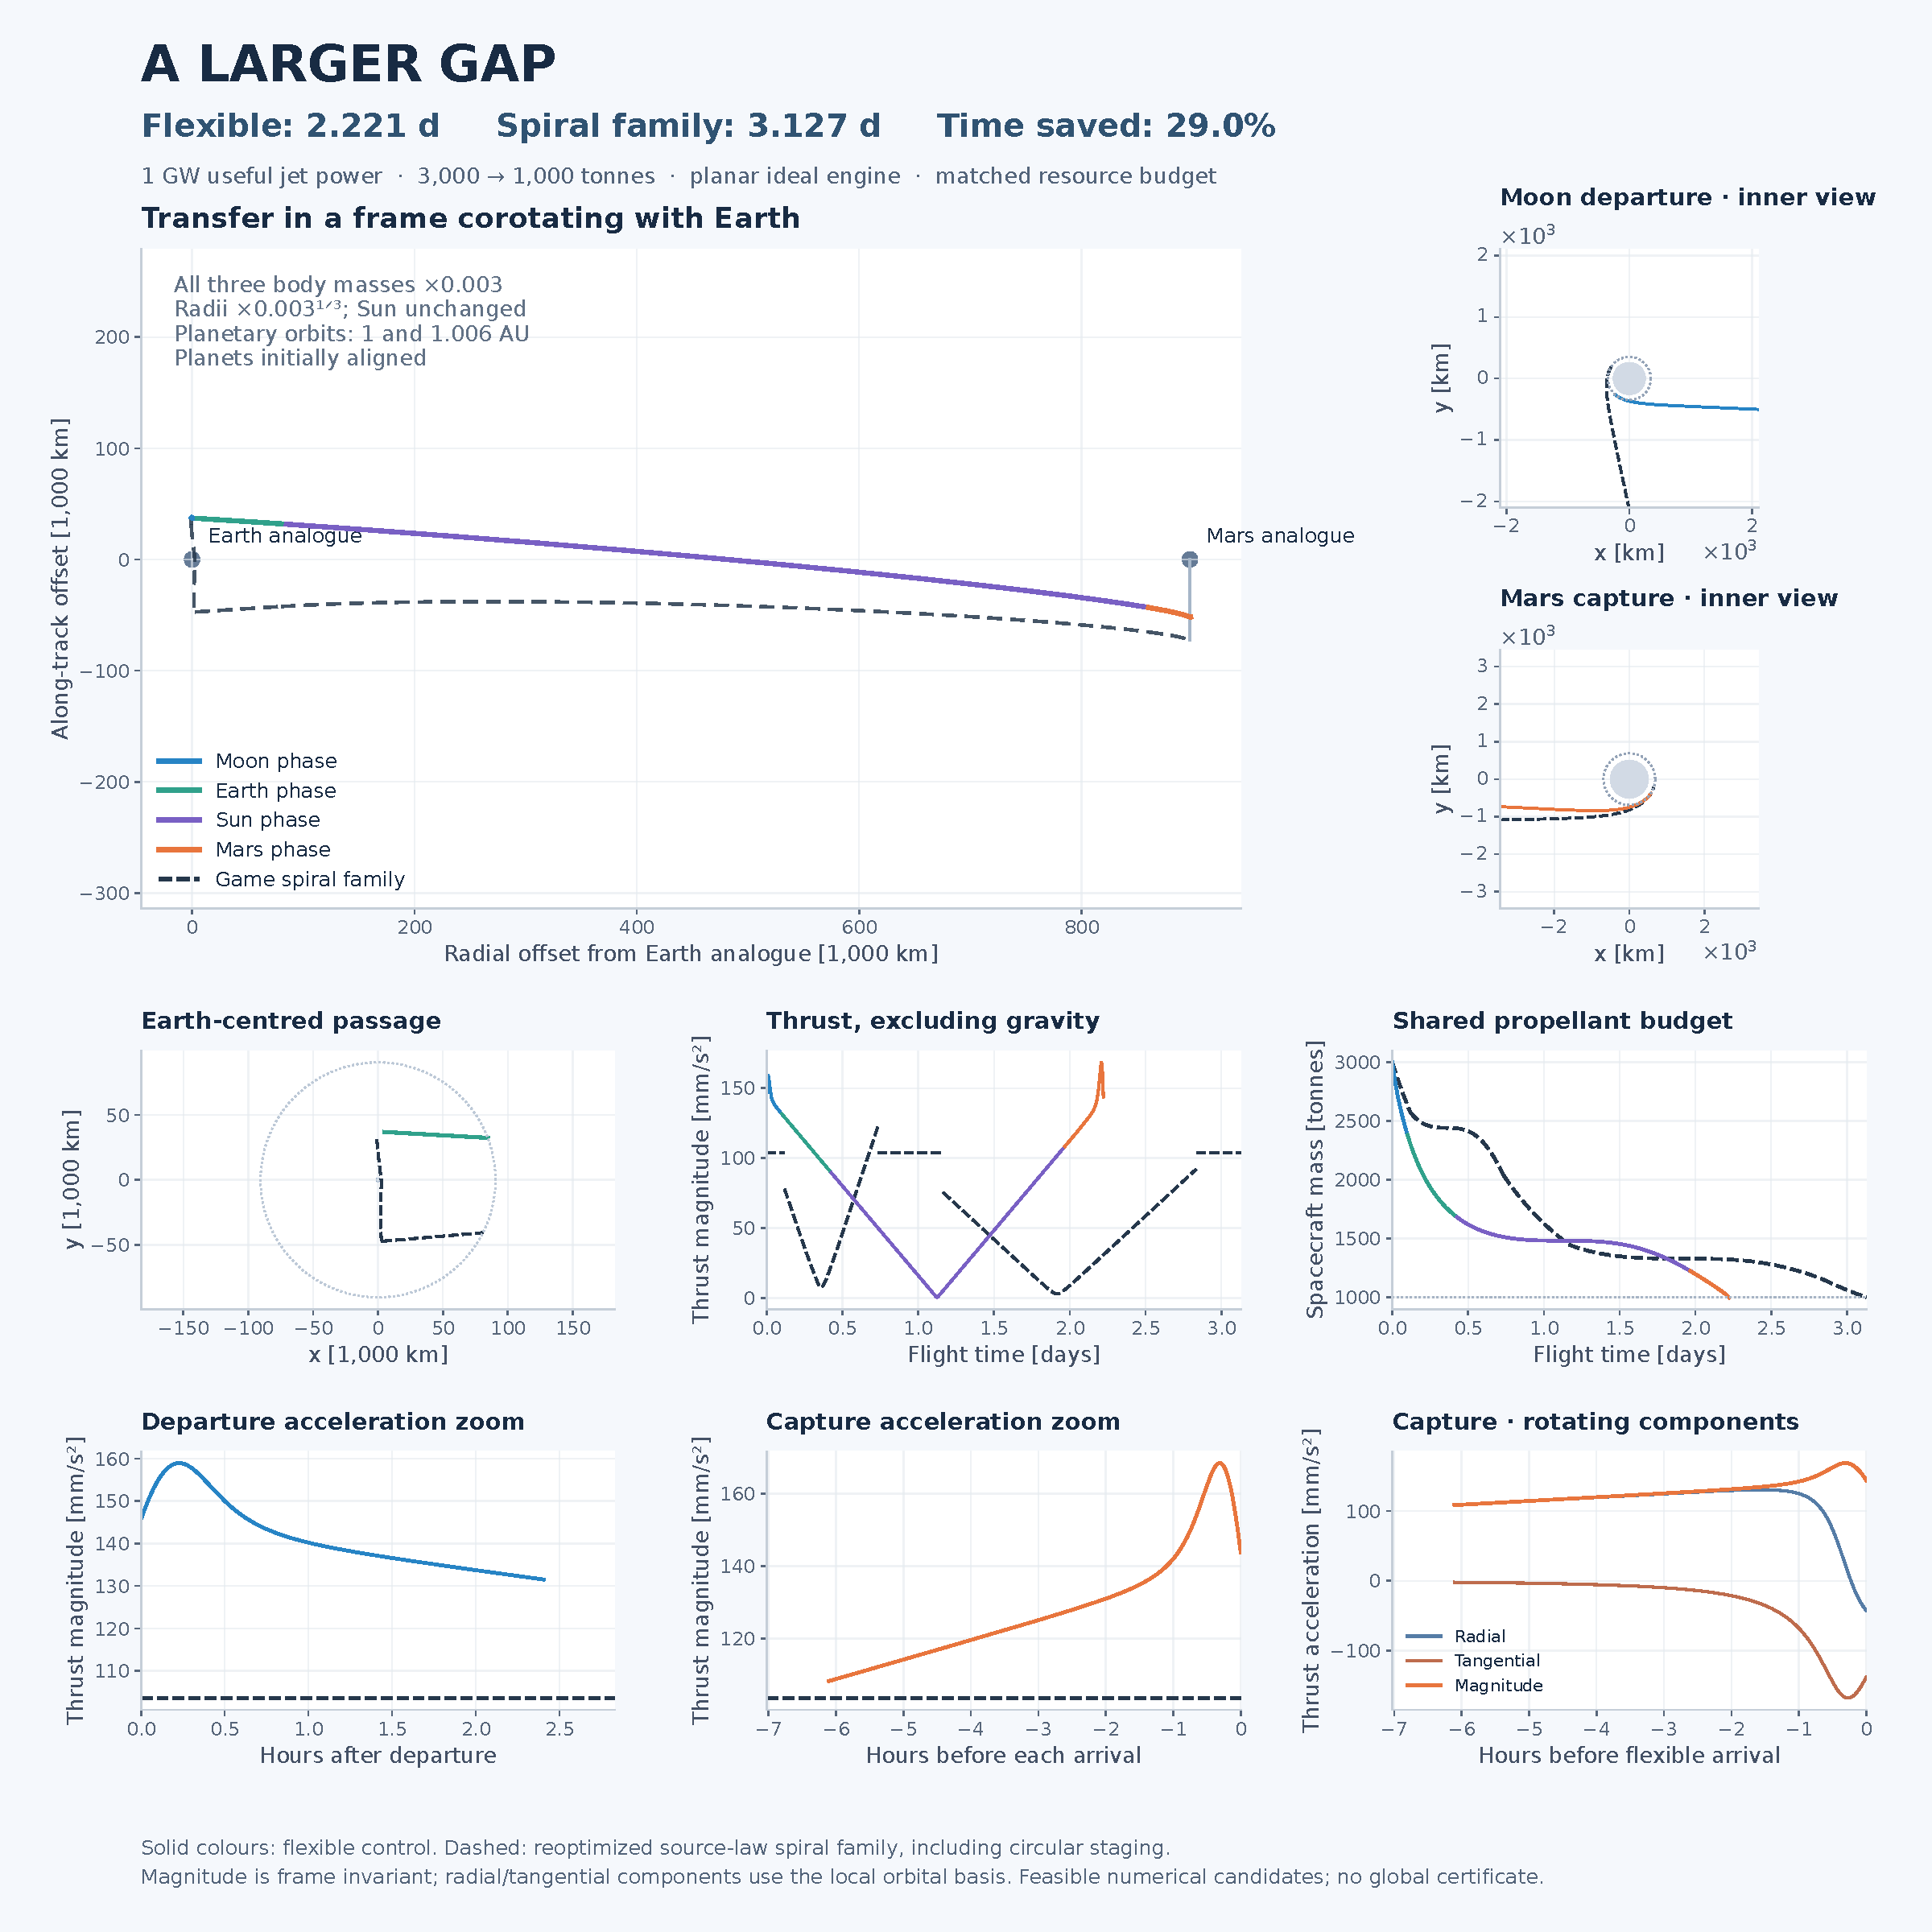
\includegraphics[width=\textwidth]{figures/large_gap_comparison.pdf}
\caption{A larger difference with the same ship in the explicitly scaled system. Nearby planetary orbits shorten the heliocentric leg and expose the cost of the staging-and-spiral restrictions. The overview is corotating; local panels are body-centred. The bottom magnitude panels cover only the respective Moon and Mars phases, aligned to departure or each method's arrival. No claim of a maximum possible performance gap is made.}
\label{fig:large-gap-comparison}
\end{figure*}

\subsection{Verification and scope of the numerical evidence}
The flexible transcription uses degree-five Radau collocation, continuous piecewise-linear local thrust components and the Sundman variable $\dd t/\dd s=r/V_{\rm ref}$. The original Moon--Mars result uses phase meshes $(300,300,160,540)$; its preceding refinement changes time by about $0.003\,\mathrm s$. The constructed case uses $(220,160,160,360)$; refinement from $(100,80,80,180)$ changes its uncorrected duration by less than $0.001\,\mathrm s$. The condensed baseline uses $(160,200)$ on its two free legs, with a refined local spiral map. Its refinement changes the uncorrected durations by less than $0.003\,\mathrm s$ in both examples.

Independent Cartesian DOP853 propagation carries the incoming state across every interface, without resetting it to an optimized endpoint. Small shooting corrections close endpoints and use the common budget, while retaining the baseline's exact constant-$A$ spiral law. The changes in flight time are approximately $-1.02$ and $-14.84\,\mathrm s$ for the Solar-System flexible and baseline candidates, and $-0.64$ and $-0.88\,\mathrm s$ for the corresponding scaled candidates. These corrections and their control changes are retained in the data. All four final checks pass: radius errors below $0.5\,\mathrm m$, radial and transverse speed errors below $0.003\,\mathrm{m\,s^{-1}}$, adequate final mass, and sampled SOI-domain and clearance checks. Small solver residuals belong to the uncorrected transcription; they are not an indirect PMP or second-variation certificate for the corrected controls.

The exploratory search tested three scaled systems. One unconverged result was rejected despite its apparently larger gap; the two converged cases gave approximately $29\%$ savings, and the larger of these was refined and plotted. Neither this search nor the two optimized trajectory families establish global optimality, a worst-case gap, or a general mission-performance guarantee. The bundle includes configurations, controls, replayed states, validation reports, refinement data and reproducible figure code.
\clearpage
\twocolumn
\setlength{\abovedisplayskip}{6pt plus 2pt minus 2pt}
\setlength{\belowdisplayskip}{6pt plus 2pt minus 2pt}
\setlength{\abovedisplayshortskip}{3pt plus 1pt minus 1pt}
\setlength{\belowdisplayshortskip}{6pt plus 2pt minus 2pt}

